\documentclass{article}
\usepackage[UKenglish]{babel}

\usepackage{graphicx}
\usepackage{booktabs}
\usepackage{multirow}
\usepackage{amsmath}
\usepackage{natbib}
\usepackage{color}

%\usepackage[paperwidth=37.75cm, paperheight=23.75cm, margin=0cm]{geometry}
\usepackage[paperwidth=174mm, paperheight=109mm, margin=0cm]{geometry}
% \renewcommand{\familydefault}{\sfdefault}
\usepackage{fontspec}
\setmainfont{Arial}
\setlength{\parindent}{0pt}

\begin{document}
\begin{tabular}{l@{}l}
  \large{A}&\hspace{1.25em}\large{B}\\
  \hspace{-0.25em}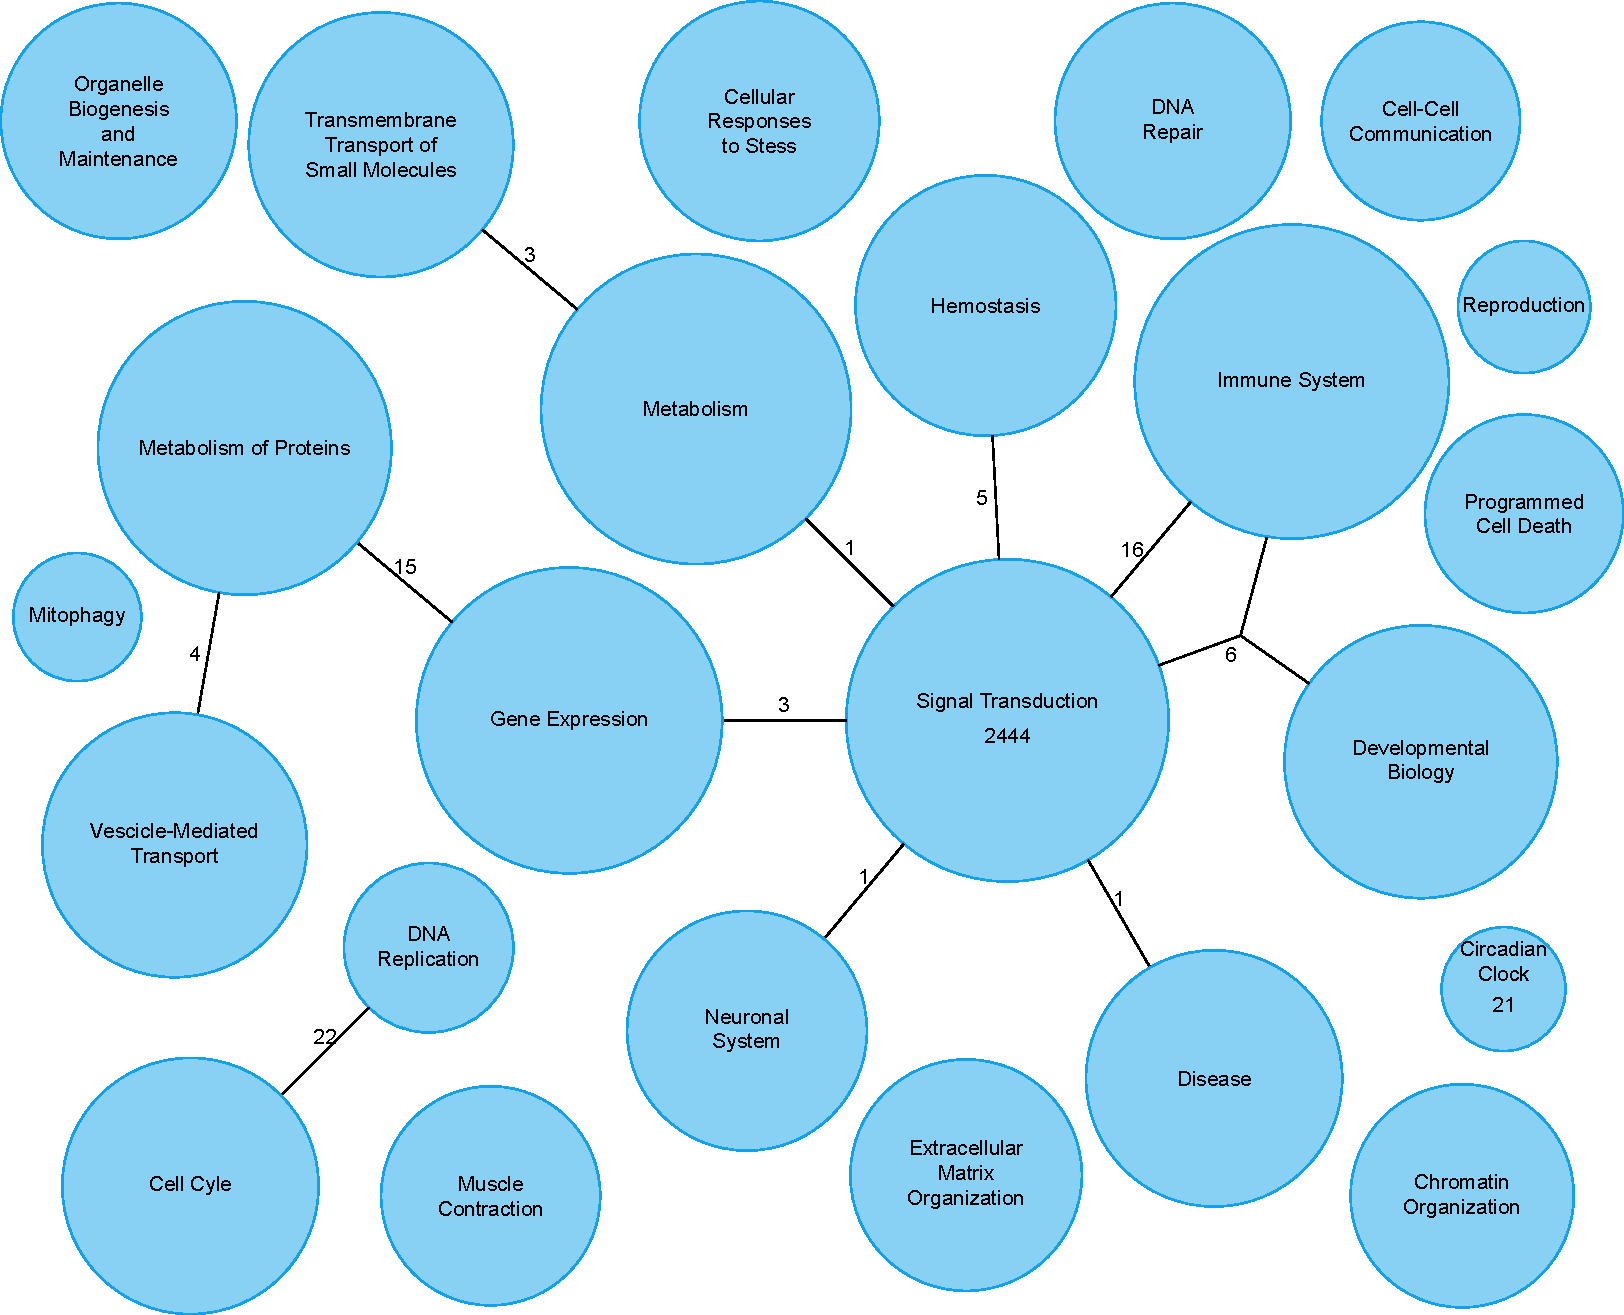
\includegraphics[scale=0.47]{Figure4a.pdf}&%
  \hspace{0.1em}%
  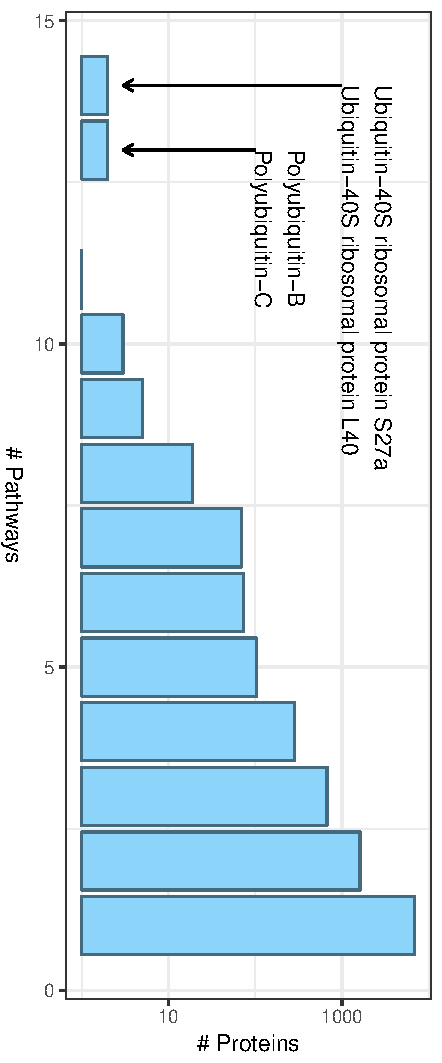
\includegraphics[scale=0.58]{Figure4b.pdf}\\
\end{tabular}

\end{document}

